\subsection{Remote Desktop}
\begin{frame}[fragile]{Connecting: Remote Desktop}
\begin{itemize}
\item First time starting a remote desktop:
\begin{semiverbatim}
\footnotesize
[sjr20@login-a-1 ~]\$ vncserver

You will require a password to access your desktops.

Password: 
Verify:   
Would you like to enter a view-only password (y/n)? n

New 'login-a-1:99 (sjr20)' desktop is login-a-1:{\color{red}99}

Starting applications specified in /home/sjr20/.vnc/xstartup
Log file is /home/sjr20/.vnc/login-a-1:99.log
\end{semiverbatim}
\item{NB Choose a \alert{different} password for VNC.}
\item{The VNC password protects your desktop from other users.}
\item{Remember the unique display number ({\color{red}99} here) of your desktop.}
\end{itemize}
\end{frame}

\begin{frame}[fragile]{Connecting: Remote Desktop}
\begin{itemize}
\item Remote desktop already running:
\begin{semiverbatim}
\footnotesize
[sjr20@login-a-1 ~]\$ vncserver -list

TigerVNC server sessions:

X DISPLAY #     PROCESS ID
:99             130655
\end{semiverbatim}
\smallskip\item Kill it:
\begin{semiverbatim}
\footnotesize
[sjr20@login-a-1 ~]\$ vncserver -kill :99
Killing Xvnc process ID 130655
\end{semiverbatim}
\smallskip\item\alert{Typically you only need {\color{red}one} remote desktop.}
\item\alert{Keeps running until killed, or the node reboots.}
\end{itemize}
\end{frame}

%\begin{frame}{TurboVNC Session}
%\begin{center}
%\centerline{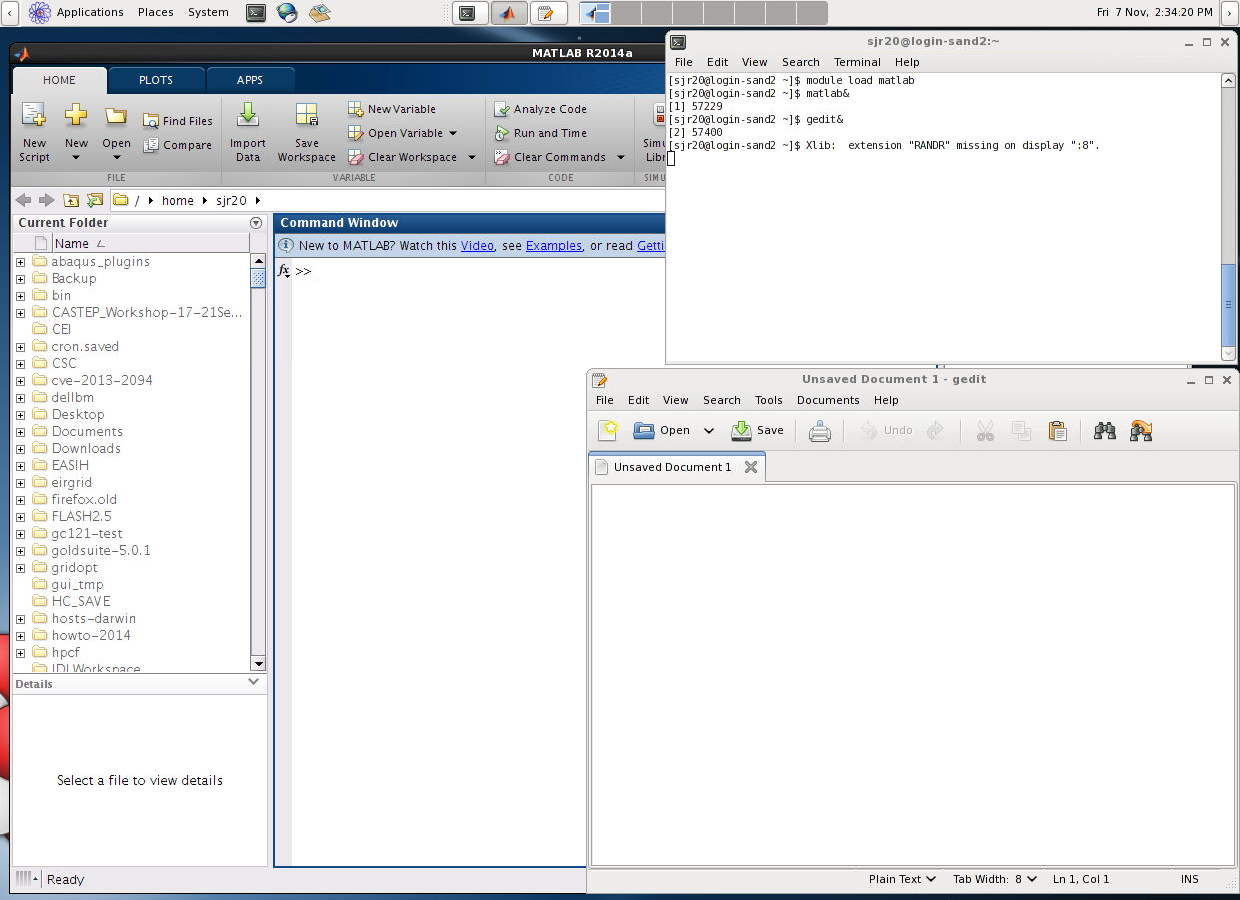
\includegraphics[width=0.85\textwidth]{imgs/linux-turbovnc.png}}
%\end{center}
%\end{frame}

%\begin{frame}{Linux TurboVNC Control Panel}
%\begin{center}
%\centerline{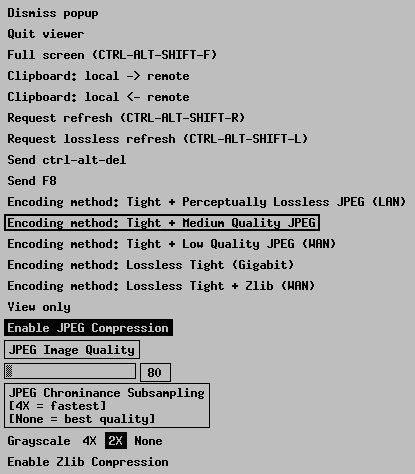
\includegraphics[height=0.8\textheight]{imgs/linux-turbovnc-F8.png}}
%\end{center}
%\end{frame}

\begin{frame}{Connecting: Remote Desktop (MobaXterm)}
\begin{center}
\centerline{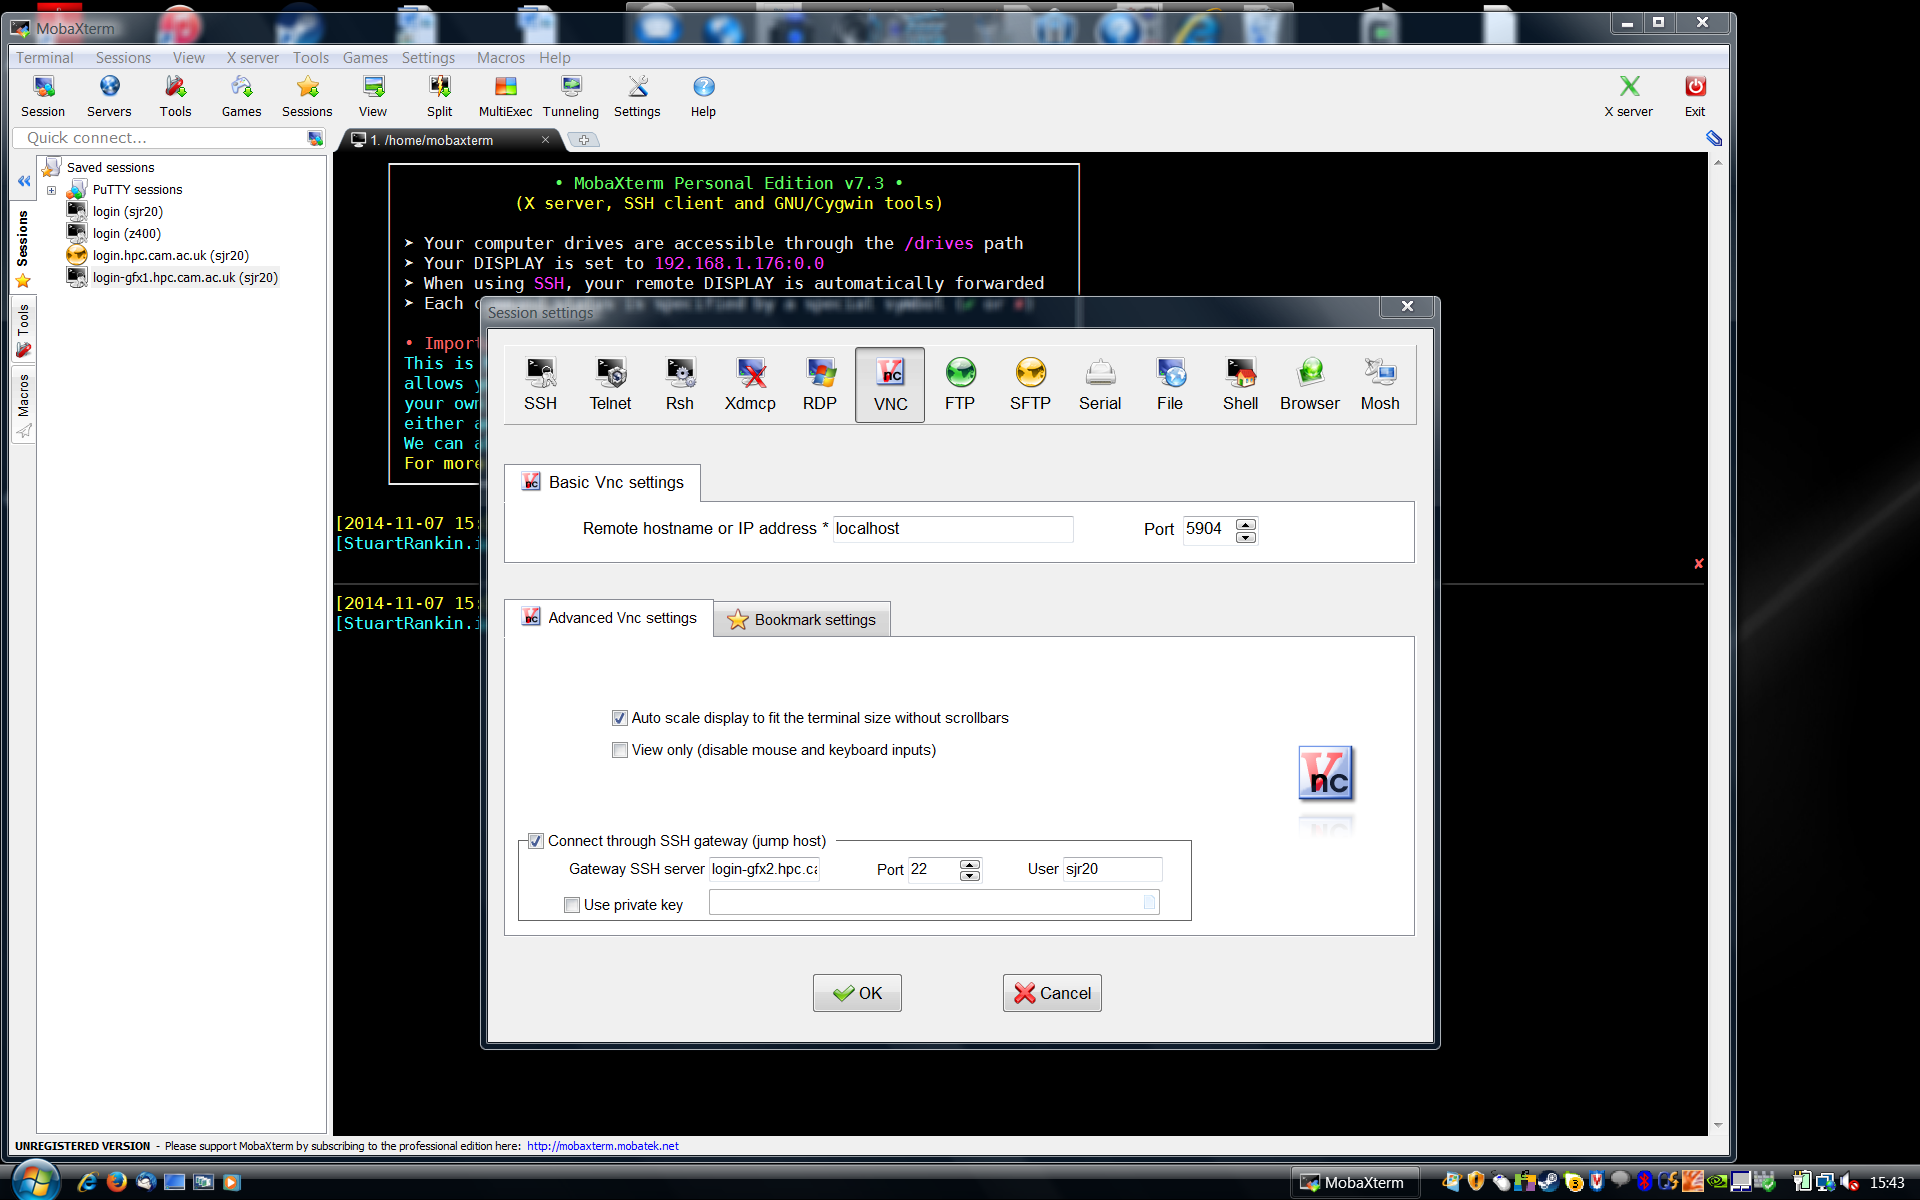
\includegraphics[height=0.8\textheight]{imgs/mobaxterm-turbovnc.png}}
\end{center}
\end{frame}